\documentclass[10pt,
               a4paper,
               journal,
               ]{IEEEtran}
\makeatletter

\def\markboth#1#2{\def\leftmark{\@IEEEcompsoconly{\sffamily}\MakeUppercase{\protect#1}}%
\def\rightmark{\@IEEEcompsoconly{\sffamily}\MakeUppercase{\protect#2}}}
\makeatother

\usepackage[utf8]{inputenc}
\usepackage[T1]{fontenc}
\usepackage{cite}
\usepackage{amsfonts}
\usepackage[pdftex]{graphicx}
\graphicspath{{../png/}}
\DeclareGraphicsExtensions{.png}
\usepackage[cmex10]{amsmath}
\interdisplaylinepenalty=2500
\usepackage{array}
\usepackage{mdwmath}
\usepackage{mdwtab}
\usepackage{eqparbox}
\usepackage[caption=false,font=footnotesize]{subfig}
\usepackage{fixltx2e}
\usepackage{stfloats}
\usepackage{url}
\hyphenation{op-tical net-works semi-conduc-tor}
\usepackage{stmaryrd}
\usepackage{bbding}
\usepackage{algpseudocode}
\usepackage{algorithm}
\usepackage{tikz}
\usetikzlibrary{shapes}
\usetikzlibrary{calc}
\usetikzlibrary{positioning}
\usetikzlibrary{patterns}
\usepackage{listings}
\usepackage{color}

\definecolor{dkgreen}{rgb}{0,0.6,0}
\definecolor{gray}{rgb}{0.5,0.5,0.5}
\definecolor{mauve}{rgb}{0.58,0,0.82}

\lstset{frame=tb,
  language=C++,
  aboveskip=3mm,
  belowskip=3mm,
  showstringspaces=false,
  columns=flexible,
  basicstyle={\small\ttfamily},
  numbers=none,
  numberstyle=\tiny\color{gray},
  keywordstyle=\color{blue},
  commentstyle=\color{dkgreen},
  stringstyle=\color{mauve},
  breaklines=true,
  breakatwhitespace=true
  tabsize=3
}

\newcommand{\reffig}[1]{{Fig.~\ref{#1}}}
\newcommand{\refeq}[1]{{(\ref{#1})}}

\begin{document}
	\title{Constraint Programming Algorithms used in Gecode}
	\author{Benedikt~Schmidt}
	\markboth{Advanced Seminar for Security in Information Technology, Summer Term 2014}%
	{Benedikt Schmidt: Constraint Programming - Inside \emph{Gecode}}	
	\maketitle	
	
	\begin{abstract}	
		Constraint programming is a method to describe and solve mathematical problems with arbitrary constraints. In the following paper, I will explain the implemented algorithms in \emph{Gecode}, a tool which can be used to solve problems through constraint programming.
	\end{abstract}
	
	\section{Introduction}
	Constraint programming is a method to solve mathematical problems through the formulation of constraints, which describe the desired solution. A formal and exact definition for constraint programming can be found in \cite[p.~16]{handbookCP}. For a better visualization of the topic, I will start with the problem of the placement of two squares such that they do not overlap.	
	
	\begin{figure}[b]
		\center
		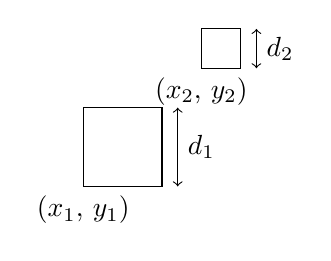
\begin{tikzpicture}
			\draw (0, 0) rectangle (1, 1);
			\node at (0, -0.3) {($x_1$, $y_1$)};
			\draw[arrows=<->] (1.2, 0) -- (1.2, 1);
			\node at (1.5, 0.5) {$d_1$};
			\draw (1.5, 1.5) rectangle(2, 2);
			\node at (1.5, 1.2) {($x_2$, $y_2$)};
			\draw[arrows=<->] (2.2, 1.5) -- (2.2, 2);
			\node at (2.5, 1.75) {$d_2$};
		\end{tikzpicture}
		\caption{Two squares which should not overlap}
		\label{fig:squares}
	\end{figure}
	
	The related variables for this example are defined in \reffig{fig:squares}. The problem can be expressed by \cite[p. 101]{programmingGecode}
	\begin{equation}
	\begin{split}
		x_1 + d_1 \le x_2 & \lor x_2 + d_2 \le x_1 \lor \\
		y_1 + d_1 \le y_2 & \lor y_2 + d_2 \le y_1
	\end{split}
	\label{eq:squares}
	\end{equation}
	The task for the constraint programming tool is to find feasible solutions which fulfill the constraints.
	
	A solver for constraint programming like \emph{Gecode} provides the necessary tools to define constraints like \refeq{eq:squares} in their most natural form as equalities and inequalities. The solver will find all possible solutions or just one of them, depending on the selected algorithm. Consequently, constraint programming with its ability to consider constraints in their most general form can be used in various fields like scheduling of resources, computer-aided design or robotics \cite[p.~221]{trendsInCP}.
	
	In the following I will explain the necessary steps to describe and solve a problem with constraint programming: variables, constraints, objective functions, search trees, constraint propagation and search algorithms. As example of an implementation I will refer to \emph{Gecode} \cite{gecode}.
	
	\section{State of the Art}
	\subsection{Variable Domains}
	In constraint programming a variable is connected to a set of possible values, the so called domain. Depending on the domain, a variable is called an integer, Boolean or floating variable. Possible ranges for a variable $x$ of each domain are:
	\begin{itemize}
		\item Integer: finite or infinite, e.g. $x \in \mathbb{N}$, $x \in \{-5, 4, 10\}$
		\item Bool: $x \in \{\text{true}, \text{false}\}$
		\item Float: intervals or unions of intervals, e.g. $x \in [-4, 3]$, $x \in [-10, 8] \cup [10, 12]$
	\end{itemize}
	This distinction is fundamental as especially for floating variables a combinatorial approach to constraint programming is impossible.
	
	\subsection{Constraint Types}
	The choice of constraint types and how comfortable it is to specify them varies from the programming language in which the problem is implemented. For sure, there is also a difference in the interfaces of the libraries for constraint programming. Typical constraints are
	\begin{itemize}
		\item Equalities: $x = y + 2$, $x^2 + y^2 = 1$, \dots
		\item Inequalities: $x \ne y$, \dots
		\item Relations: $x < 2 y$, $e^x < 4$, \dots
	\end{itemize}
	
	Different constraint types can also be combined, for example inequalities or equalities through logic operators to Boolean expressions. Some of these constraints may acquire special attention during the search for solutions to improve the runtime of the search. For this reason a lot of work has been done for example on the alldifferent constraint \cite{allDifferent}
	\begin{equation}
		\forall x_i, x_j \in D, i \ne j: x_i \ne x_j, 
		\label{eq:alldifferent}
	\end{equation}
	which is an example for a combined constraint.
	
	\subsection{Objective Functions}
	A constraint problem can have, additional to constraints, an objective function. As in optimization only one objective function can be optimized at a time, a problem in constraint programming must have either one or no objective function. To solve problems with an objective function it is necessary to select a search algorithm which is capable of optimization.
	
	\subsection{Search Trees}
	
	\begin{figure}
		\center
		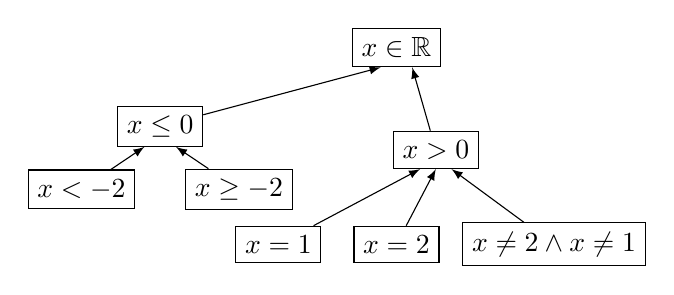
\begin{tikzpicture}
			\tikzstyle{arrow}=[draw, -latex]
			\node[rectangle,draw] at (0, 2) (levelOne) {$x \in \mathbb{R}$};
			
			\node[rectangle,draw] at (-3, 1) (levelTwoElementOne) {$x \le 0$};
			\coordinate[left=0.2cm of levelOne.south] (levelOnePointOne);
	  		\path[arrow] (levelTwoElementOne) -- (levelOnePointOne);
	  		
			\node[rectangle,draw] at (0.5, 0.7) (levelTwoElementTwo) {$x > 0$};
			\coordinate[right=0.2cm of levelOne.south] (levelOnePointTwo);
	  		\path[arrow] (levelTwoElementTwo) -- (levelOnePointTwo);
	  		
			\node[rectangle,draw] at (-4, 0.2) (levelThreeElementOne) {$x < -2$};
			\coordinate[left=0.2cm of levelTwoElementOne.south] (levelTwoElementOnePointOne);
	  		\path[arrow] (levelThreeElementOne) -- (levelTwoElementOnePointOne);
	  		
			\node[rectangle,draw] at (-2, 0.2) (levelThreeElementTwo) {$x \ge -2$};
			\coordinate[right=0.2cm of levelTwoElementOne.south] (levelTwoElementOnePointTwo);
	  		\path[arrow] (levelThreeElementTwo) -- (levelTwoElementOnePointTwo);
	  		
			\node[rectangle,draw] at (-1.5, -0.5) (levelThreeElementThree) {$x = 1$};
			\coordinate[left=0.2cm of levelTwoElementTwo.south] (levelTwoElementTwoPointOne);
	  		\path[arrow] (levelThreeElementThree) -- (levelTwoElementTwoPointOne);
	  		
			\node[rectangle,draw] at (0, -0.5) (levelThreeElementFour) {$x = 2$};
			\coordinate[right=0cm of levelTwoElementTwo.south] (levelTwoElementTwoPointTwo);
	  		\path[arrow] (levelThreeElementFour) -- (levelTwoElementTwoPointTwo);
	  		
			\node[rectangle,draw] at (2, -0.5) (levelThreeElementFive) {$x \ne 2 \land x \ne 1$};
			\coordinate[right=0.2cm of levelTwoElementTwo.south] (levelTwoElementTwoPointThree);
	  		\path[arrow] (levelThreeElementFive) -- (levelTwoElementTwoPointThree);
		\end{tikzpicture}
		\caption{search tree on one variable $x$}
		\label{fig:searchTree}
	\end{figure}
	
	In constraint programming, search trees, like the one in \reffig{fig:searchTree}, describe the partition of the search space. Their nodes have names, depending on their position in the tree. The search is started from the root node. At this point, all variable domains are still complete. The root node is also the first one with a branch, where the search space is split up into disjoint sets. This approach is based on the same idea like the divide-and-conquer technique \cite[p.~175]{artOfComputerProgramming}, as it reduces a complex problem into two or more parts with less complexity. The splitting, which adds additional constraints on the variables, is then recursively done with different heuristics to partition the search space into smaller parts. If one of the parts is small enough to decide if it is feasible the node can be called a either a dead end or a solution. To end up as a dead end, there must be no feasible solutions left in the search space at this node. To turn the node into a solution it is necessary that all members of the reduced search space are valid considering the constraints. This can be the case if either only one choice is left for every variable, and the constraints are valid for this choice, or if a whole interval of a floating variable is valid for the constraints.
	
	\subsection{Constraint Propagation}
	Constraint propagation is a key concept in constraint programming as it reduces the size of the search space significantly. The term propagation refers in this area to the reduction of choices for variables which are infeasible, considering other constraints and affected variable domains. As the size of the variable domain is related to the possibilities which have to be checked by a search through additional subtrees, the constraint propagation is able to prune complete infeasible subtrees. Therefore, the whole search process can be accelerated through constraint propagation.
	
	\begin{figure}
		\center
		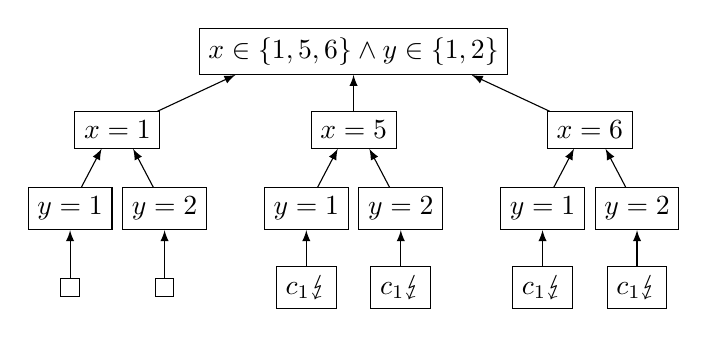
\begin{tikzpicture}
			\tikzstyle{arrow}=[draw, -latex]
			\node[rectangle,draw] at (0, 3) (levelOne) {$x \in \{1, 5, 6\} \land y \in \{1, 2\}$};
			
			\node[rectangle,draw] at (-3, 2) (levelTwoElementOne) {$x = 1$};
			\coordinate[left=1.5cm of levelOne.south] (levelOnePointOne);
	  		\path[arrow] (levelTwoElementOne) -- (levelOnePointOne);
	  		
			\node[rectangle,draw] at (0, 2) (levelTwoElementTwo) {$x = 5$};
			\coordinate[left=0cm of levelOne.south] (levelOnePointTwo);
	  		\path[arrow] (levelTwoElementTwo) -- (levelOnePointTwo);
	  		
			\node[rectangle,draw] at (3, 2) (levelTwoElementThree) {$x = 6$};
			\coordinate[right=1.5cm of levelOne.south] (levelOnePointThree);
	  		\path[arrow] (levelTwoElementThree) -- (levelOnePointThree);
	  		
			\node[rectangle,draw] at (-3.6, 1) (levelThreeElementOne) {$y = 1$};
			\coordinate[left=0.2cm of levelTwoElementOne.south] (levelTwoElementOnePointOne);
	  		\path[arrow] (levelThreeElementOne) -- (levelTwoElementOnePointOne);
			\node[rectangle,draw] at (-3.6, 0) (levelFourElementOne) {\Checkmark};
	  		\path[arrow] (levelFourElementOne) -- (levelThreeElementOne);
			\node[rectangle,draw] at (-2.4, 1) (levelThreeElementTwo) {$y = 2$};
			\coordinate[right=0.2cm of levelTwoElementOne.south] (levelTwoElementOnePointTwo);
	  		\path[arrow] (levelThreeElementTwo) -- (levelTwoElementOnePointTwo);
			\node[rectangle,draw] at (-2.4, 0) (levelFourElementTwo) {\Checkmark};
	  		\path[arrow] (levelFourElementTwo) -- (levelThreeElementTwo);
	  		
			\node[rectangle,draw] at (-0.6, 1) (levelThreeElementThree) {$y = 1$};
			\coordinate[left=0.2cm of levelTwoElementTwo.south] (levelTwoElementTwoPointOne);
	  		\path[arrow] (levelThreeElementThree) -- (levelTwoElementTwoPointOne);
			\node[rectangle,draw] at (-0.6, 0) (levelFourElementThree) {$c_1 \lightning$};
	  		\path[arrow] (levelFourElementThree) -- (levelThreeElementThree);
			\node[rectangle,draw] at (0.6, 1) (levelThreeElementFour) {$y = 2$};
			\coordinate[right=0.2cm of levelTwoElementTwo.south] (levelTwoElementTwoPointTwo);
	  		\path[arrow] (levelThreeElementFour) -- (levelTwoElementTwoPointTwo);
			\node[rectangle,draw] at (0.6, 0) (levelFourElementFour) {$c_1 \lightning$};
	  		\path[arrow] (levelFourElementFour) -- (levelThreeElementFour);
	  		
			\node[rectangle,draw] at (2.4, 1) (levelThreeElementFive) {$y = 1$};
			\coordinate[left=0.2cm of levelTwoElementThree.south] (levelTwoElementThreePointOne);
	  		\path[arrow] (levelThreeElementFive) -- (levelTwoElementThreePointOne);
			\node[rectangle,draw] at (2.4, 0) (levelFourElementFive) {$c_1 \lightning$};
	  		\path[arrow] (levelFourElementFive) -- (levelThreeElementFive);
			\node[rectangle,draw] at (3.6, 1) (levelThreeElementSix) {$y = 2$};
			\coordinate[right=0.2cm of levelTwoElementThree.south] (levelTwoElementThreePointTwo);
	  		\path[arrow] (levelThreeElementSix) -- (levelTwoElementThreePointTwo);
			\node[rectangle,draw] at (3.6, 0) (levelFourElementSix) {$c_1 \lightning$};
	  		\path[arrow] (levelFourElementSix) -- (levelThreeElementSix);
		\end{tikzpicture}
		\caption{search tree without constraint propagation}
		\label{fig:bigTree}
	\end{figure}
	
	\begin{figure}
	\center
	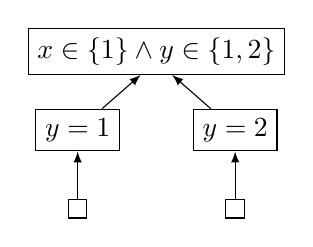
\begin{tikzpicture}
		\tikzstyle{arrow}=[draw, -latex]
		\node[rectangle,draw] at (0, 2) (levelOne) {$x \in \{1\} \land y \in \{1, 2\}$};
  		
		\node[rectangle,draw] at (-1, 1) (levelTwoElementOne) {$y = 1$};
		\coordinate[left=0.2cm of levelOne.south] (levelOnePointOne);
  		\path[arrow] (levelTwoElementOne) -- (levelOnePointOne);
		\node[rectangle,draw] at (-1, 0) (levelThreeElementOne) {\Checkmark};
  		\path[arrow] (levelThreeElementOne) -- (levelTwoElementOne);
		\node[rectangle,draw] at (1, 1) (levelTwoElementTwo) {$y = 2$};
		\coordinate[right=0.2cm of levelOne.south] (levelOnePointTwo);
  		\path[arrow] (levelTwoElementTwo) -- (levelOnePointTwo);
		\node[rectangle,draw] at (1, 0) (levelThreeElementTwo) {\Checkmark};
  		\path[arrow] (levelThreeElementTwo) -- (levelTwoElementTwo);
	\end{tikzpicture}
	\caption{search tree with constraint propagation}
	\label{fig:smallTree}
	\end{figure}
	
	To illustrate this effect consider a problem based on two variables $x \in \{1, 5, 6\}$ and $y \in \{1, 2\}$ and the constraint
	\begin{equation}
		c_1:\ x \le y
	\end{equation}
	Without constraint propagation and branching first on $x$, a decision, which may have been made by a certain branching strategy, the search trees turns out to be the one in \reffig{fig:bigTree}. By inspection one sees that the right parts of this tree can be already pruned at the root by propagation of constraint $c_1$. Therefore, it is not necessary to create and evaluate these subtrees. With constraint propagation fewer branches have to be made, like it can be seen in \reffig{fig:smallTree}.
	
	The implementation of constraint propagation is different in each tool. However, the same principles are used. In this paper, I will describe the \emph{Gecode} implementation.
	
	Constraints in \emph{Gecode} are evaluated ahead of a further growth of a subtree, as it may be possible to prune some of the subtrees. The problem here is to decide in which order the constraints should be considered, and it may even be necessary to evaluate some constraints more often. A short example will illustrate this \cite[p.~575]{handbookCP}: Let there be two constraints 
	\begin{equation}
		c_1: y - x^2 = 0
	\end{equation}
	\begin{equation}
		c_2: y - x - 1 = 0
		\label{eq:linear}
	\end{equation}
	and let the variable domains be $x, y \in [-4, 4]$. Starting with the evaluation of constraint $c_1$ follows a chain of reductions of the variable domains, based only on constraint propagation:
	\begin{equation}
	\begin{split}
		c_1:\ &y \in [-4, 4] \rightarrow y \in [0, 4] \\
		c_1:\ &x \in [-4, 4] \rightarrow x \in [-2, 2] \\
		c_2:\ &y \in [0, 4] \rightarrow y \in [0, 3] \\
		c_2:\ &x \in [-2, 2] \rightarrow x \in [-1, 2] \\
		c_1:\ &x \in [-1, 2] \rightarrow x \in [-1, 1.73 \dots] \\
		&\dots
	\end{split}
	\end{equation}
	
	To implement this repeated evaluation of constraints in \emph{Gecode} all constraints subscribe to the domains of the variables which are part of them. A more detailed explanation of this observer pattern can be found in \cite{designPatterns}. With this method, the constraints get notified whenever a variable domain is reduced and they can signal the system that they need to be evaluated once again.
	
	The next decision to be made is which constraint should be evaluated first. In the example above the constraints were quite simple and therefore it would not make a big difference to evaluate first $c_1$ or $c_2$, the search will take nearly the same time. Unfortunately, not all constraints are equally fast to evaluate and for this case \emph{Gecode} defines for every constraint a certain cost \cite[p.~275]{programmingGecode}. Based on this cost the constraints are sorted into buckets which are then evaluated in order of ascending cost. This means, whenever a variable domain is changed, the first try is to use constraints with the lowest possible cost and only if none of them needs to be evaluated constraints with higher costs are considered.
	
		\subsection{Branching Strategies}
	If at one node it is not possible to empty one variable domain or to reduce all variable domains to the size of one it is necessary to make a decision: How should the next subtree be constructed? The question is answered by the selected branching strategy. No matter which one is selected, they all have in common that they create additional, temporary constraints, which are only applied to the specific subtrees. This process is called \emph{posting} a constraint on a branch.
	
	The branching strategy depends on the variable domain: For integer variables there are three common strategies \cite[p.~87]{handbookCP} which differ in how the domain is distributed to the subtrees.
	\begin{itemize}
		\item Enumeration: The domain for $x \in D = {x_1, x_2, \dots}$ is split up into $|D|$-branches where for every branch $i$ one additional constraint $c:\ x = x_i$ is posted.
		\item Binary choice points: One value $x_i$ from the domain $D$ of the variable $x$ is selected and the domain is split up into two subtrees: On one the constraint $x = x_i$ and on the other one the constraint $x \ne x_i$ is posted. This results into something similar to a binary tree at this point.
		\item Domain splitting: The domain $D$ for the variable $x$ is split up into two disjoint intervals or sets, for example $x < 2$ and $x \ge 2$.
	\end{itemize}
	
	As for variables with a float domain the enumeration and binary choice points are not feasible, the last one, domain splitting, is typically used. As termination criteria for a float it is necessary to define a certain epsilon $\epsilon > 0$ which describes the interval length, at which the solver states to have found a solution.
	
	For branching strategies there is a choice of freedom left, for instance where the interval is split up, and this freedom can be used to implement some heuristics. This additional information is either gained during the search itself or predefined by the user.
	
	\subsection{Search Algorithms}
	Search algorithms define the way the search tree is constructed and traversed, starting from the root node. To improve the performance of the search at every node a constraint propagation is executed, which may narrow the search space down. Then, based on these two steps, either one, the best or no solution is found. The actual result of the search depends on the type of the search algorithm.
	
	In \emph{Gecode} it is possible to define custom strategies. However, the user is supported at this point with some standard algorithms which he can use to build custom ones:
	\begin{itemize}
		\item Depth-first search
		\item Limited discrepancy search
		\item Branch-and-bound search
		\item Depth-first search restart optimization
	\end{itemize}
	
	In the following part I will discuss the depth-first search, the branch-and-bound search, the limited discrepancy search as candidate for an improved backjumping-strategy, backjumping strategies in general and restart strategies.
	
	\subsubsection{Depth-First Search}
	The idea behind this search algorithm is that every possible combination of variables is examined. In its basic form it can not be applied to problems with infinite domains; for problems with such variable domains it is necessary to use for instance branch-and-bound. Sometimes the depth-first search is also referred to as chronological backtrack search.
	
	The starting point for the depth-first search is the root node, from where on the algorithm is called recursively. At every node, mainly two steps are executed: First, a constraint propagation to reduce the variable domains and second a branching, which divides the search space into two disjoint subspaces, on which the same algorithm is applied again. The search stops in a leaf of the search tree if either no branching is possible and therefore a valid solution is found, or one or more variable domains are emptied, which indicates that in this leave no possible solution exists.
	
	This search is a so-called complete algorithm as it can be proven that all possible solutions will be found \cite[p.~85]{handbookCP}. Because of this characteristic it is very useful to prove for example that for a certain problem no solution exists. The main drawback is the execution time, as it does an exhaustive search. Maybe even the memory usage can become a problem if during the search many solutions are found.
	
	By stopping the search after the first feasible solution is found the runtime of the search can be improved. Although this slightly modified version is not complete anymore, in practice it is in some areas sufficient to know just one valid solution.
	
	\subsubsection{Depth-First Search with Optimization}
	If in the constraint programming an objective is defined which should be either minimized or maximized, a modified version of the depth-first search can be applied. The only difference is that it evaluates the objective function for every found solution concerning the constraints and stores during the search only the best one. To accelerate the search it is possible to add an additional constraint which requires that the new value for the objective must be better than the best achieved so far. Through this enhancement even more subtrees are pruned and the search is faster.
	
	This algorithm is also complete. Hence, it will always find the best solution, if one exists. This algorithm does not inherit the bad memory characteristics from the depth-first search as only one solution is stored, but the search is still exhaustive and can be very slow, depending on the size of the variable domains.
	
	\subsubsection{Branch-and-Bound Search}
	A branch-and-bound search is an algorithm for optimization of an objective function under certain constraints and only discrete possible candidates for a solution. The difference to the depth-first search with optimization is the usage of a so-called relaxed optimum, the optimum without consideration of the required discreetness.
	
	During a branch-and-bound search two steps are executed: branch-and-reduce and bounding. The first one partitions the search space and the second one prunes whole areas with non-optimal solutions.
	
	\begin{figure}
		\center
		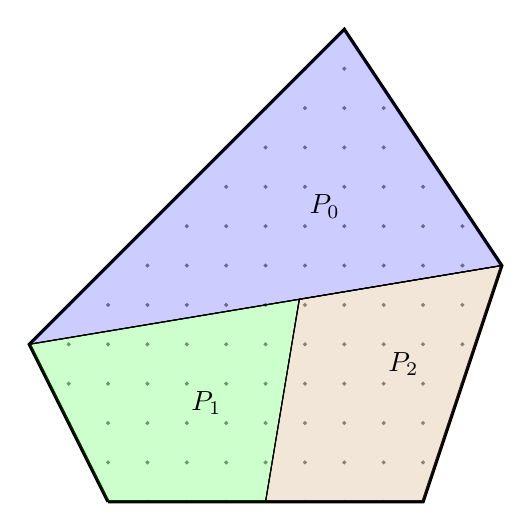
\begin{tikzpicture}
			\coordinate (a) at (0, 0);
			\coordinate (b) at (4, 0);
			\coordinate (c) at (5, 3);
			\coordinate (d) at (3, 6);
			\coordinate (e) at (-1, 2);
			\coordinate (f) at (2, 0);
			\coordinate (g) at (intersection of e--c and f--d);
			
			\begin{scope}
				\clip (a) -- (b) -- (c) -- (d) -- (e) -- (a);
				\foreach \x in {-2,-1.5,...,5}
				{
	      			\foreach \y in {0,0.5,...,6}
	      			{
	        			\node[draw,circle,inner sep=0.2pt,fill,gray] at (\x,\y) {};
	      			}
	    		}
    		\end{scope}
			
			\draw[very thick] (a) -- (b) -- (c) -- (d) -- (e) -- (a);
			\draw (a) -- (b) -- (c) -- (e) -- (a);
			\draw (f) -- (g) -- (c) -- (b) -- (f);
			\draw[fill=blue, fill opacity=0.2] (c) -- (d) -- (e) -- (c);
			\draw[fill=green, fill opacity=0.2] (a) -- (f) -- (g) -- (e) -- (a);
			\draw[fill=brown, fill opacity=0.2] (f) -- (g) -- (c) -- (b) -- (f);
			\node at (2.75, 3.75) {$P_0$};
			\node at (1.25, 1.25) {$P_1$};
			\node at (3.75, 1.75) {$P_2$};
		\end{tikzpicture}	
		\caption{Splitting of a search space into three subproblems and the possible candidates for solutions}
		\label{fig:branchAndBound}
	\end{figure}
	
	The basic concept for finding solutions in branch-and-bound is an enumeration of all possible candidates. Therefore, it is necessary to separate the search space in an appropriate way, which is the task for the branch-and-reduce step. This step is very similar to the concept of branching, it also depends on a certain heuristic to divide the search space into two or even more disjoint parts. This heuristic can either be selected by the user or be a general one, like splitting the biggest variable domain into two equal sized parts. If the basic search space contains a big amount of possible candidate solutions one reduction may not be enough and therefore this step is applied recursively to the newly create subproblems. This process can be stopped if the number of solutions is reduced to an amount, where it is possible to enumerate all of them and check if they are optimal. A possible division into subproblems can be seen in \reffig{fig:branchAndBound}, where for legibility branch-and-reduce was applied only twice: The first execution split the problem into $P_0$ and $P'_0$, which was then split again into $P_1$ and $P_2$.
	
	The next step after branch-and-reduce is the bounding, which is able to prune whole subproblems. In the following part I will consider the minimization of an objective function without a loss of generality:
	\begin{equation}
		\max_x \{f(x)\} = -\min_x \{-f(x)\}
	\end{equation}
	
	For the bounding it is first necessary to initialize a upper bound with a value, for example with $\infty$. This upper bound is updated during the process every time a new optimal solution is found to this new optimum. If a new possible solution is found which is above this upper bound the algorithm can prune it, as only the minimum solution is of interest. 
	
	The actual pruning of subproblems is based on the relaxed optimum, which is the optimum of the problem without consideration that only discrete values are allowed. If this relaxed optimum for a certain subproblem is greater than the current upper bound it is possible to prune this complete subproblem, as it can not contain a better solution.
	
	Consider for this \reffig{fig:branchAndBound}, where already a certain optimum $f$ was found in subproblem $P_1$. If now the relaxed optimum $f_{P0}$ in $P_0$ and $f_{P2}$ in $P_2$ is worse than this optimum
	\begin{equation}
		f_{P0} > f
	\end{equation}
	\begin{equation}
		f_{P2} > f
	\end{equation}
	the whole subproblems $P_{0}$ and $P_{2}$ can be pruned and it is not necessary to enumerate the solution candidates in them (or to split them further up).
	
	Combined with appropriate branching the bounding can prune several candidates at once, without the necessity to enumerate them. Therefore bounding is able to improve the performance of the search.
	
	\subsubsection{Limited Discrepancy Search}
	The limited discrepancy search falls into the category of best-first searches and was first mentioned by Harvey and Ginsberg \cite{limitedDiscrepancy}. It depends on branching heuristics for the tree, which are determined through branching strategies. The basic concept is that during a chronological backtrack search a wrong turn close to the root is first of all very expensive. Second, heuristics work worse the farther away from the solution they are applied. Therefore, decisions close to the root node are likely to fail. Consequently, in a depth-first search the worst decisions are the most expensive ones. The limited discrepancy search solves exactly this problem as it suggests to change rather the decisions made close to the root than the ones the search made later. The improvement compared to a chronological backtrack was shown by experimental results and theoretically proven in \cite{limitedDiscrepancy}.
	
	\subsubsection{Backjumping}
	A specific version of backjumping was already mentioned, the limited discrepancy search, where instead of jumping one node back the algorithm always jumps as far back to the root node as possible. In general this is proven to be better than the chronological backtracking \cite{limitedDiscrepancy}. However, for certain problems it may be possible to find better nodes to jump back. A jump back in the search tree means to detect a so-called nogood decision, which caused the violation of a constraint in the dead end. How these nogoods must be selected and stored to improve the search depends heavily on the specific field and if it is done wrong the backjumping can even be less efficient than chronological backtracking \cite[p.~100]{handbookCP}.
	
	\subsubsection{Restart Strategies}
	Branching always means to apply certain heuristics and these heuristics may fail or produce bad results for the first execution of the search algorithm. If it turns out that the search tree is build in a disadvantageous way a restart strategy may be appropriate to improve the search. For such a restart the heuristic is improved, based on the things the search has learned to be a not so good solution during the first or first few attempts to build a search tree.
	For practical application several variants of restart strategies were proposed \cite[p.~113]{handbookCP}.
	
	\section{Conclusion}
	\emph{Gecode}, as representative for an implementation of constraint programming, provides the necessary tools to describe and solve a wide range of combinatorial or optimization problems. The interface allows an adaption to the area of application through modifications of algorithms, restarts or the implementation of a custom search algorithm, based on the already provided ones. Therefore, \emph{Gecode} can be used in various areas, starting from scheduling, over portfolio optimization up to technical problems like placement.
	
	\begin{thebibliography}{1}
		\bibitem{handbookCP}
		F.~Rossi, P.~van~Beek and T.~Walsh, \emph{Handbook of Constraint Programming}, Amsterdam, The Netherlands: Elsevier, 2006, ISBN-13: 978-0-444-52726-4
		\bibitem{allDifferent}
		W.~van~Hoeve, \emph{The Alldifferent Constraint: A Survey}, http://www.andrew.cmu.edu/user/vanhoeve/papers/alldiff.pdf
		\bibitem{trendsInCP}
		F.~Benhamou, N.~Jussien, B.~A.~O'Sullivan, \emph{Trends in Constraint Programming}, Wiley-ISTE, 2007, ISBN-13: 978-1-905209-97-2
		\bibitem{gecode}
		http://www.gecode.org/
		\bibitem{programmingGecode}
		C.~Schulte, G.~Tack and M.~Z.~Lagerkvist, \emph{Modeling and Programming with Gecode}, http://www.gecode.org/doc-latest/MPG.pdf
		\bibitem{limitedDiscrepancy}
		W.~D.~Harvey, M.~L.~Ginsberg, \emph{Limited Discrepancy Search}, Morgan Kaufmann, 1995
		\bibitem{linearProgramming}
		L.~Cooper and D.~Steinberg, \emph{Methods and Applications of Linear Programming}, W.~B.~Saunder~Company, 1974, ISBN-10: 0-7216-2694-7
		\bibitem{artOfComputerProgramming}
		D.~E.~Knuth, \emph{The Art of Computer Programming: Volume 3, Sorting and Searching}, second edition, Addison-Wesley, 1998, ISBN-10: 0201896850, ISBN-13: 9780201896855
		\bibitem{designPatterns}
		E.~Gamma, R.~Helm, R.~Johnson, J.~Vlissides, \emph{Design Patterns. Elements of Reusable Object-Oriented Software}, first edition, Prentice Hall, 1994, ISBN-10: 0201633612
	\end{thebibliography}
\end{document}


